\documentclass[dvipsnames, tikz]{standalone}
\usepackage{amsmath}
\usepackage{arevmath}
\usepackage{xcolor}
\usepackage{tikz}
\usetikzlibrary{calc}
\usetikzlibrary{decorations.pathreplacing,calligraphy,3d}
\usetikzlibrary{matrix,shapes,fit,backgrounds}

\tikzset{main/.style={color=black, line join=round}}

\begin{document}
	\begin{tikzpicture}
		\clip (-2.2,-2.9) rectangle ++(8.4,5);
		\draw[thick, main, fill=BrickRed] (0,0) --++(1,0) --++(120:1) -- cycle;	
	\end{tikzpicture}

	\begin{tikzpicture}
		\clip (-2.2,-2.9) rectangle ++(8.4,5);
		\draw[thick, main, fill=BrickRed] (0,0) --++(1,0) --++(120:1) -- cycle;
		\draw[thick, main, fill=BurntOrange] (1,0) --++(60:1) --++(180:1) -- cycle;
	\end{tikzpicture}

	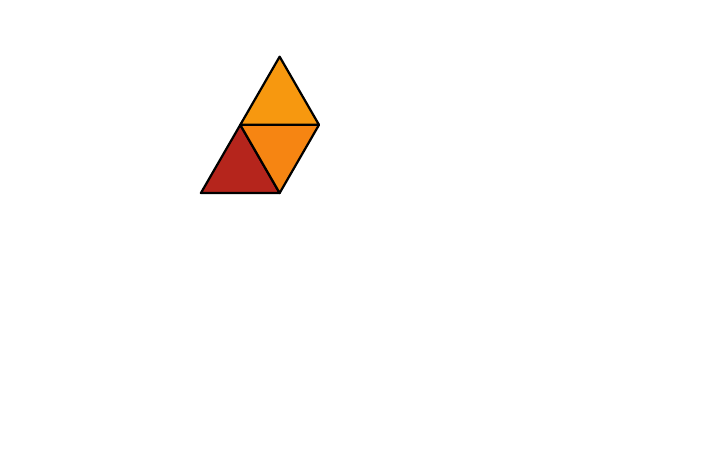
\begin{tikzpicture}
		\clip (-2.2,-2.9) rectangle ++(8.4,5);
		\draw[thick, main, fill=BrickRed] (0,0) --++(1,0) --++(120:1) -- cycle;
		\draw[thick, main, fill=BurntOrange] (1,0) --++(60:1) --++(180:1) -- cycle;
		\draw[thick, main, fill=YellowOrange] (60:1) --++(1,0) --++(120:1) -- cycle;
	\end{tikzpicture}

	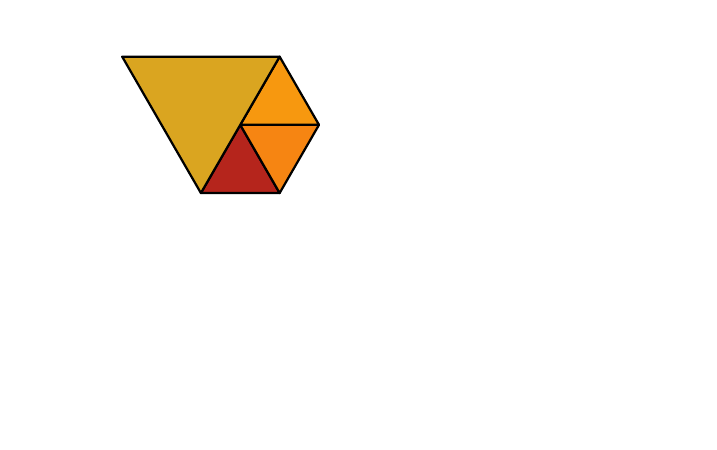
\begin{tikzpicture}
		\clip (-2.2,-2.9) rectangle ++(8.4,5);
		\draw[thick, main, fill=BrickRed] (0,0) --++(1,0) --++(120:1) -- cycle;
		\draw[thick, main, fill=BurntOrange] (1,0) --++(60:1) --++(180:1) -- cycle;
		\draw[thick, main, fill=YellowOrange] (60:1) --++(1,0) --++(120:1) -- cycle;
		\draw[thick, main, fill=Goldenrod] (0,0) --++(60:2) --++(180:2) -- cycle;
	\end{tikzpicture}

	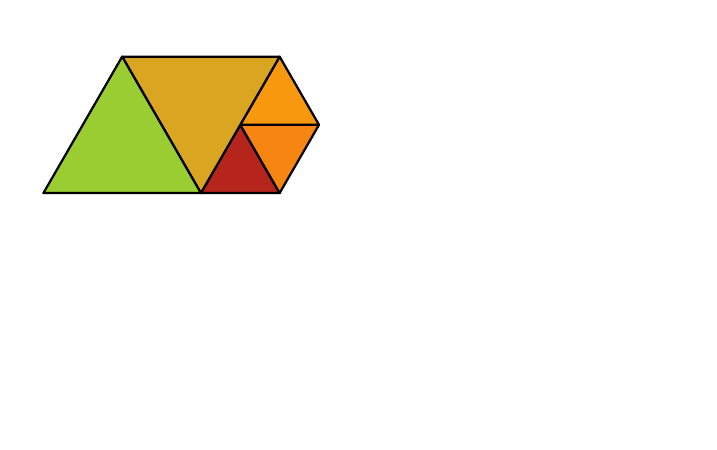
\begin{tikzpicture}
		\clip (-2.2,-2.9) rectangle ++(8.4,5);
		\draw[thick, main, fill=BrickRed] (0,0) --++(1,0) --++(120:1) -- cycle;
		\draw[thick, main, fill=BurntOrange] (1,0) --++(60:1) --++(180:1) -- cycle;
		\draw[thick, main, fill=YellowOrange] (60:1) --++(1,0) --++(120:1) -- cycle;
		\draw[thick, main, fill=Goldenrod] (0,0) --++(60:2) --++(180:2) -- cycle;
		\draw[thick, main, fill=YellowGreen] (0,0) --++(120:2) --++(240:2) -- cycle;
	\end{tikzpicture}

	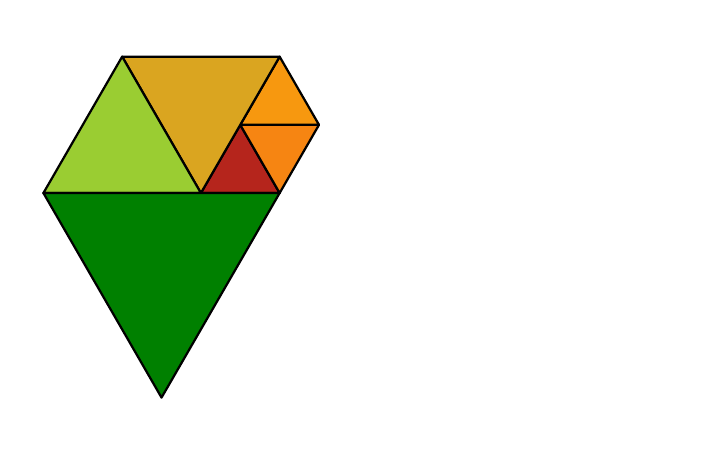
\begin{tikzpicture}
		\clip (-2.2,-2.9) rectangle ++(8.4,5);
		\draw[thick, main, fill=BrickRed] (0,0) --++(1,0) --++(120:1) -- cycle;
		\draw[thick, main, fill=BurntOrange] (1,0) --++(60:1) --++(180:1) -- cycle;
		\draw[thick, main, fill=YellowOrange] (60:1) --++(1,0) --++(120:1) -- cycle;
		\draw[thick, main, fill=Goldenrod] (0,0) --++(60:2) --++(180:2) -- cycle;
		\draw[thick, main, fill=YellowGreen] (0,0) --++(120:2) --++(240:2) -- cycle;
		\draw[thick, main, fill=Green] (-2,0) --++(-60:3) --++(60:3) -- cycle;
	\end{tikzpicture}

	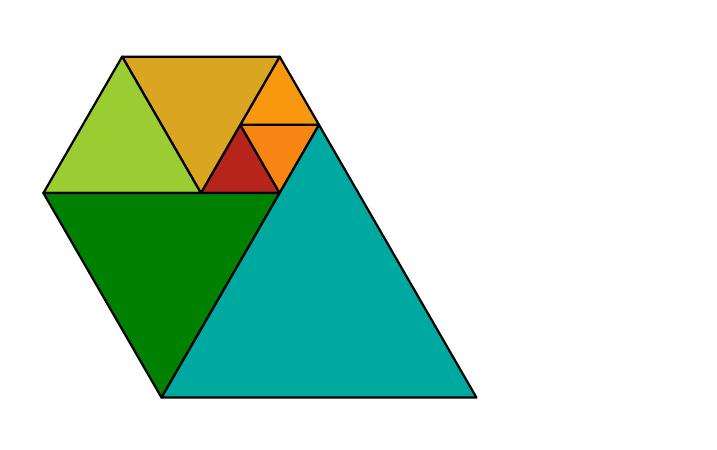
\begin{tikzpicture}
		\clip (-2.2,-2.9) rectangle ++(8.4,5);
		\draw[thick, main, fill=BrickRed] (0,0) --++(1,0) --++(120:1) -- cycle;
		\draw[thick, main, fill=BurntOrange] (1,0) --++(60:1) --++(180:1) -- cycle;
		\draw[thick, main, fill=YellowOrange] (60:1) --++(1,0) --++(120:1) -- cycle;
		\draw[thick, main, fill=Goldenrod] (0,0) --++(60:2) --++(180:2) -- cycle;
		\draw[thick, main, fill=YellowGreen] (0,0) --++(120:2) --++(240:2) -- cycle;
		\draw[thick, main, fill=Green] (-2,0) --++(-60:3) --++(60:3) -- cycle;
		\draw[thick, main, fill=Emerald] (1,0) ++ (60:1) --++(-60:4) --++(180:4) -- cycle;
	\end{tikzpicture}
	
	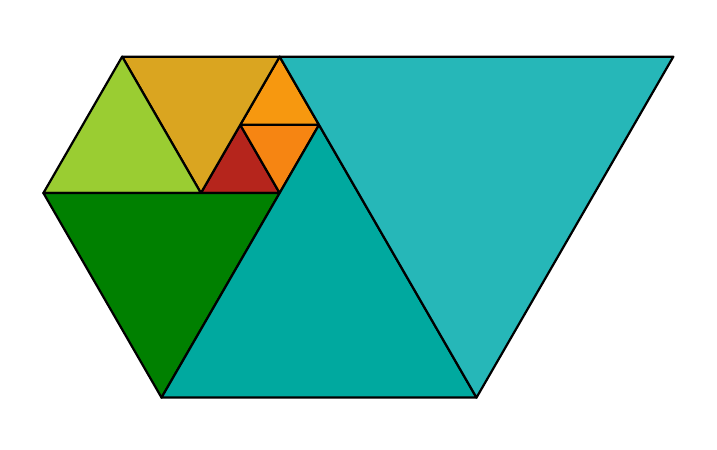
\begin{tikzpicture}
		\clip (-2.2,-2.9) rectangle ++(8.4,5);
		\draw[thick, main, fill=BrickRed] (0,0) --++(1,0) --++(120:1) -- cycle;
		\draw[thick, main, fill=BurntOrange] (1,0) --++(60:1) --++(180:1) -- cycle;
		\draw[thick, main, fill=YellowOrange] (60:1) --++(1,0) --++(120:1) -- cycle;
		\draw[thick, main, fill=Goldenrod] (0,0) --++(60:2) --++(180:2) -- cycle;
		\draw[thick, main, fill=YellowGreen] (0,0) --++(120:2) --++(240:2) -- cycle;
		\draw[thick, main, fill=Green] (-2,0) --++(-60:3) --++(60:3) -- cycle;
		\draw[thick, main, fill=Emerald] (1,0) ++ (60:1) --++(-60:4) --++(180:4) -- cycle;
		\draw[thick, main, fill=BlueGreen] (60:2) --++(-60:5) --++(60:5) -- cycle;
	\end{tikzpicture}
\end{document}